%=====================================================================
%  Q-learning vs SARSA on warehouse robot navigation
%  Build:  ./build.sh   (three pdflatex passes; clears stale auxiliaries)
%
%  NOTE: this TeX installation has no array, booktabs, geometry, xcolor,
%  titlesec, caption or listings, and no TS1 text-symbol fonts. Margins are
%  therefore set by hand, tables use plain tabular, the booktabs rules are
%  aliased to \hline, and the itemize label and underscore are redefined
%  via \char. Do not add those packages back without checking kpsewhich.
%=====================================================================
\documentclass[11pt,a4paper,oneside]{report}

\usepackage{amsmath,amssymb,amsfonts}
\usepackage{graphicx}
\usepackage{longtable}
\usepackage{url,verbatim,color,calc,ifthen,alltt}
\usepackage[hidelinks]{hyperref}

% ---- page geometry (the geometry package is unavailable) --------------------
\setlength{\oddsidemargin}{0.10in}
\setlength{\evensidemargin}{0.10in}
\setlength{\textwidth}{6.20in}
\setlength{\topmargin}{-0.30in}
\setlength{\headheight}{14pt}
\setlength{\headsep}{20pt}
\setlength{\textheight}{9.15in}
\setlength{\parskip}{4pt}
\setlength{\parindent}{0pt}

% ---- booktabs-style rules (booktabs is unavailable) -------------------------
\newcommand{\toprule}{\hline}
\newcommand{\midrule}{\hline}
\newcommand{\bottomrule}{\hline}
\renewcommand{\arraystretch}{1.25}

% ---- TS1 fonts are absent: supply these from the base encodings -------------
\newcommand{\bs}{\char`\\}
\newcommand{\us}{\char`\_}
\renewcommand{\labelitemi}{$\bullet$}
\renewcommand{\labelitemii}{$\circ$}

\definecolor{accent}{rgb}{0.165,0.471,0.839}
\definecolor{warm}{rgb}{0.922,0.408,0.204}

\newcommand{\code}[1]{\texttt{\small #1}}
\newcommand{\keypoint}[1]{\par\vspace{3pt}\noindent\textbf{#1}}

\hyphenation{Q-learn-ing SARSA ware-house ex-plo-ra-tion}

\begin{document}

%=====================================================================
\begin{titlepage}
\centering
\vspace*{0.6in}

{\Large\bfseries On-Policy and Off-Policy Temporal-Difference Control\\[6pt]
for Warehouse Robot Navigation}\\[10pt]

{\large A controlled comparison of Q-learning and SARSA,\\
implemented from first principles and evaluated over thirty paired seeds}\\[0.5in]

\rule{\textwidth}{0.8pt}\\[0.25in]

{\large\textbf{Case Study Report}}\\[6pt]
{\large Reinforcement Learning}\\[6pt]
{\large Smart Warehouse Robot Navigation --- learning the shortest\\
collision-free delivery route}\\[0.3in]

\rule{\textwidth}{0.8pt}\\[0.5in]

\begin{tabular}{rl}
\textbf{Research question} & How do Q-learning and SARSA compare when a robot must\\
                           & learn the shortest collision-free route to a delivery point?\\[8pt]
\textbf{Dataset}           & \code{zoya77/robot-path-planning-navigation-dataset}\\
                           & 7{,}980 warehouse snapshots; 5{,}045 distinct 5$\times$5 layouts\\[8pt]
\textbf{Algorithms}        & Q-learning (off-policy) and SARSA (on-policy),\\
                           & both written from scratch in NumPy\\[8pt]
\textbf{Protocol}          & 30 paired seeds per algorithm, identical budget,\\
                           & Wilcoxon signed-rank on the paired differences\\
\end{tabular}

\vfill
{\large Source code and executed notebook:}\\[4pt]
\url{https://github.com/Ashwin-3cS/transformer-t1}\\[0.3in]
{\large \today}
\end{titlepage}

\pagenumbering{roman}
\setcounter{page}{2}

\chapter*{Abstract}
\addcontentsline{toc}{chapter}{Abstract}

This report presents a controlled empirical comparison of the two classical tabular
temporal-difference control algorithms --- Q-learning, which is off-policy, and SARSA, which is
on-policy --- on the problem of learning a collision-free delivery route across a warehouse floor.
Both algorithms are implemented from first principles, sharing every component except the single
expression that forms their update target, so that the comparison isolates the on-policy/off-policy
distinction rather than any difference of implementation.

Obstacle layouts are taken from a published Kaggle dataset of warehouse navigation grids. A column
by column audit of that dataset is reported as part of the methodology, because several of its
columns prove to carry no usable information: its reward signal correlates $-0.03$ with the true
shortest-path distance, its path-length field correlates $+0.01$, its convergence flag is constant,
and its episode identifiers do not describe coherent trajectories. Those fields are excluded with
the evidence shown. What remains sound --- 5{,}045 distinct occupancy grids with valid start and
goal cells --- is used to build the environment, and exact ground truth is obtained by
breadth-first search computed independently.

The report is explicit about the boundary between data and assumption. The racking layout is real.
The reward structure, the cross-aisle and the pedestrian walkway that constitutes the hazard are
declared modelling choices, and the hazard penalty is subsequently varied across a sweep because
the principal finding depends on it.

Thirteen numerical checks verify the environment and both agents before any experiment is run,
including an equivalence test establishing that at $\varepsilon = 0$ the two algorithms produce
bit-identical action-value tables, as the mathematics requires.

The experiment uses thirty seeds per algorithm, paired so that both algorithms see identical
conditions, and reports Wilcoxon signed-rank tests with bootstrap confidence intervals. The
results reproduce the classical prediction with large and highly significant effects. Q-learning
converges on the optimal 19-step route running directly alongside the walkway, achieving a mean
deployed route of 19.40 steps, but accumulates 21{,}626 safety incidents during training. SARSA
learns a route averaging 33.34 steps at more than five times the distance from the walkway, and
accumulates 5{,}068 incidents --- a factor of 4.3 fewer --- with significantly better online
return ($p = 1.9\times10^{-9}$).

Two further results qualify the finding. A sweep of the hazard penalty shows Q-learning's
behaviour to be completely invariant to it, while SARSA's clearance from the walkway rises
monotonically as the penalty grows: the mechanism is visible directly in the measurements. And on
a floor without a localised hazard, both algorithms converge on the identical optimum, confirming
that the distinction is a response to a property of the task rather than a general ranking of the
two algorithms.

\vspace{8pt}
\noindent\textbf{Keywords:} reinforcement learning, temporal-difference control, Q-learning, SARSA,
on-policy and off-policy learning, warehouse robotics, safe exploration, Cliff Walking.

\tableofcontents
\listoffigures
\listoftables

\clearpage
\pagenumbering{arabic}
\setcounter{page}{1}

\chapter{Introduction}
\label{ch:intro}

\section{Background}

A modern fulfilment warehouse is a shared workspace. Automated mobile robots move stock between
racking and packing stations while people walk the same floor, and the robot's routing problem is
therefore not only about finding the shortest path. It is about finding the shortest path that is
also safe to execute, and about doing so without causing harm during the period in which it is
still learning.

That last qualification is easy to overlook and is the subject of this report. A policy learned in
a simulator can be evaluated purely on its final quality, because mistakes made during training
cost nothing. A policy learned on a live warehouse floor cannot: every exploratory action is taken
in the real world, and the cost of learning is a cost the operator actually pays.

Reinforcement learning offers two classical algorithms for this class of problem, and they differ
precisely on this point. Q-learning \cite{watkins1989,watkins1992} learns the value of the optimal
policy regardless of how the agent is behaving. SARSA \cite{rummery1994,sutton1996} learns the
value of the policy the agent is actually following, exploration included. On a benign problem the
two converge to the same answer. On a problem where exploration can be costly they do not, and the
difference is both predictable and practically important.

\section{Problem statement}

The task is navigation on a warehouse floor represented as a grid. A robot starts at a charging
station and must reach a delivery point. Racking blocks movement. A pedestrian walkway crosses the
floor, and entering it is a safety incident.

The shortest route runs along the main aisle, which lies directly alongside the walkway. A second
route one row further from the walkway is slightly longer and carries no such exposure. The
problem is interesting because those two routes differ in exactly the way that distinguishes the
two algorithms: the fast route is optimal for an agent that never makes mistakes, and dangerous
for one that is still exploring.

\section{Research question}

\begin{quote}
\textbf{How do Q-learning and SARSA compare when a warehouse robot must learn the shortest
collision-free route to a delivery point?}
\end{quote}

Four subsidiary questions are answered empirically:

\begin{enumerate}
\item \textbf{Deployed quality.} After training, which algorithm's greedy policy produces the
      shorter route, and how close is it to the true optimum?
\item \textbf{Cost of learning.} Which algorithm accumulates fewer safety incidents while learning,
      and what does training cost in accumulated reward?
\item \textbf{Significance.} Are the observed differences distinguishable from seed-to-seed noise?
\item \textbf{Mechanism.} Whatever is observed, what property of the algorithms and of the task
      accounts for it?
\end{enumerate}

\section{Objectives}

\begin{enumerate}
\item Implement a grid-world warehouse environment from first principles, with no reinforcement
      learning library.
\item Implement Q-learning and SARSA from first principles, sharing all machinery except the
      update target, so that the comparison isolates the on-policy/off-policy distinction.
\item Audit the source dataset column by column and use only what carries signal, documenting the
      exclusions with evidence.
\item Verify the environment and both agents numerically before any experiment is run.
\item Compare the algorithms over thirty paired seeds with a paired non-parametric significance
      test and reported effect sizes.
\item Test the robustness of the result against an external baseline, against independently
      generated floors, and against the main modelling assumption.
\end{enumerate}

\section{Scope and delimitations}

\keypoint{Tabular methods only.} The state space is 400 cells, small enough to enumerate. Nothing
here concerns function approximation or deep reinforcement learning, where off-policy bootstrapping
raises stability issues that do not arise in the tabular case.

\keypoint{A simulated environment built on real layouts.} This point is developed at length in
Chapter~\ref{ch:dataset} because it determines what the study can honestly claim. The obstacle
layouts come from the dataset; the dynamics and the reward structure are written here.

\keypoint{One task family.} All results concern grid navigation with a localised hazard. The
report is explicit about which findings depend on that structure.

\keypoint{No tuning contest.} Both algorithms share one hyperparameter setting. The objective is
a controlled comparison, not the best achievable performance from either.

\section{Contributions}

\begin{enumerate}
\item \textbf{A documented dataset audit} showing that several columns of a published Kaggle
      dataset --- its reward signal, its path lengths, its episode structure --- carry no usable
      information, with the evidence rather than the assertion.
\item \textbf{A verification suite for tabular RL}, including an equivalence test that pins the
      two algorithms to each other under a greedy policy, where they are mathematically identical.
\item \textbf{A properly paired multi-seed comparison}, with significance testing and effect
      sizes, rather than a single run per algorithm.
\item \textbf{An explicit separation of what is data from what is assumed}, together with a
      sensitivity analysis over the assumption that drives the result.
\item \textbf{A negative control}: the demonstration that on a floor without a localised hazard,
      the two algorithms converge on the identical optimum and the much-cited distinction between
      them simply does not appear.
\end{enumerate}

\section{Organisation}

Chapter~\ref{ch:literature} reviews temporal-difference control and the on-policy/off-policy
distinction. Chapter~\ref{ch:theory} develops the mathematics: Markov decision processes, the
Bellman equations, TD(0), the two control algorithms and their convergence conditions.
Chapter~\ref{ch:dataset} audits the dataset and specifies the environment, separating data from
assumption. Chapter~\ref{ch:implementation} presents the implementation.
Chapter~\ref{ch:verification} presents the verification suite. Chapter~\ref{ch:results} reports the
experiment. Chapter~\ref{ch:discussion} interprets it and states the threats to validity.
Chapter~\ref{ch:conclusion} concludes.

\chapter{Literature Review}
\label{ch:literature}

\section{Overview}

This chapter traces the development of value-based reinforcement learning up to the two algorithms
compared here, and then examines what is and is not well established about the difference between
them. The organising question throughout is: \emph{whose} value is the agent learning?

\section{Markov decision processes and dynamic programming}

The formal setting is the Markov decision process, developed by Bellman \cite{bellman1957} and
given its modern treatment by Puterman \cite{puterman1994}. An MDP specifies states, actions,
transition probabilities and rewards, and the Markov property asserts that the next state depends
only on the current state and action.

Dynamic programming --- policy iteration and value iteration --- solves an MDP exactly, but
requires the transition and reward functions to be known in advance. A warehouse robot does not
have them. It has only the ability to act and observe what follows, which is the setting
reinforcement learning addresses.

\section{Monte Carlo and temporal-difference learning}

Two families of method learn from experience alone. Monte Carlo methods wait until an episode
terminates and update toward the observed return; they are unbiased but high-variance, and cannot
learn from incomplete episodes.

Temporal-difference learning, introduced by Sutton \cite{sutton1988}, instead updates toward a
\emph{bootstrapped} estimate --- the immediate reward plus the discounted value of the successor
state. TD methods learn online, from incomplete episodes, with far lower variance. The cost is
bias, since the target depends on the current estimate, which is itself wrong. Convergence results
for TD(0) under suitable step-size conditions are given by Dayan \cite{dayan1992} and
Jaakkola et al.\ \cite{jaakkola1994}.

The practical importance of this trade-off is that TD control learns \emph{while the robot is
still moving}, which is what makes the cost of exploration a measurable quantity in this study.

\section{Q-learning}

Q-learning, introduced by Watkins \cite{watkins1989} and proved convergent by Watkins and Dayan
\cite{watkins1992}, is the canonical \emph{off-policy} TD control algorithm. Its update
bootstraps from the maximum over next-state action values,
\[
Q(s,a) \leftarrow Q(s,a) + \alpha\Big[r + \gamma \max_{a'} Q(s',a') - Q(s,a)\Big],
\]
and this maximisation is what makes it off-policy: the target describes the greedy policy,
irrespective of the policy that generated the data. Given sufficient exploration and a suitable
step-size schedule, $Q$ converges to the optimal action-value function $Q^{*}$ regardless of how
the agent behaves while learning.

That independence is the algorithm's defining strength and, in the setting studied here, the source
of its characteristic weakness: because the target never refers to the behaviour policy, the cost
of the agent's own exploration never enters its estimates.

\section{SARSA}

SARSA was introduced by Rummery and Niranjan \cite{rummery1994} and named by Sutton
\cite{sutton1996} after the quintuple $(s,a,r,s',a')$ its update consumes:
\[
Q(s,a) \leftarrow Q(s,a) + \alpha\Big[r + \gamma Q(s',a') - Q(s,a)\Big],
\qquad a' \sim \pi(\cdot \mid s').
\]
Here $a'$ is the action the agent will actually take. The update therefore evaluates the behaviour
policy itself, making SARSA \emph{on-policy}. Under an $\varepsilon$-greedy policy, SARSA converges
to the optimal $\varepsilon$-greedy policy rather than to the optimal policy, and converges to
$Q^{*}$ only if $\varepsilon$ is decayed to zero appropriately --- the GLIE conditions
\cite{singh2000}.

This apparent weakness is the source of its practical strength. By evaluating the policy that
includes exploration, SARSA accounts for the possibility that the next action is random, and
therefore assigns lower value to states from which a random action would be catastrophic.

\section{The Cliff Walking result}

The clearest demonstration of the distinction is Example 6.6 of Sutton and Barto \cite{sutton2018},
\emph{Cliff Walking}. An agent crosses a grid from start to goal; a row of cliff cells lies between
them. Stepping into the cliff incurs a large penalty and returns the agent to the start.

The optimal path runs immediately alongside the cliff. Q-learning learns exactly that path, and
consequently falls off repeatedly while exploring, so its online performance during learning is
poor. SARSA learns a longer path further from the edge, because its estimates price in the
possibility of an $\varepsilon$-greedy step over it, and achieves better online return. Decaying
$\varepsilon$ makes both converge to the optimal policy.

Three features of this result are essential and are reproduced deliberately in the present study:

\begin{itemize}
\item The hazard is \textbf{localised and adjacent to the optimal path}. Without this there is no
      decision to make and the two algorithms behave identically.
\item The environment is \textbf{deterministic}. The effect is caused by $\varepsilon$-greedy
      exploration alone, not by stochastic dynamics.
\item The comparison measures \textbf{two distinct quantities} --- online return during learning,
      and the quality of the final greedy policy --- which have different answers.
\end{itemize}

The third point is the one most often lost in secondary accounts, which tend to report that
``SARSA is safer'' without noting that Q-learning's final policy is the better one.

\section{Related developments}

Expected SARSA \cite{vanseijen2009} replaces the sampled $Q(s',a')$ with its expectation under the
policy, reducing variance while remaining on-policy; it subsumes both algorithms as special cases.
Double Q-learning \cite{hasselt2010} addresses the maximisation bias that the $\max$ operator
introduces. Neither is evaluated here, since the object of study is the basic on-policy/off-policy
contrast, but both are natural extensions (Chapter~\ref{ch:conclusion}).

The distinction acquires additional importance under function approximation, where off-policy
bootstrapping combined with approximation and bootstrapping forms the ``deadly triad''
\cite{sutton2018} and can diverge outright. In the tabular setting studied here both algorithms
are convergent, so the difference observed is about the \emph{policy being evaluated} and not
about stability.

\section{Reinforcement learning for warehouse robots}

Automated guided vehicles and autonomous mobile robots in warehouses are a well-established
application area, and safety around human co-workers is a recognised constraint rather than an
afterthought. The field of safe reinforcement learning, surveyed by Garc\'ia and Fern\'andez
\cite{garcia2015}, is explicitly concerned with the problem this report measures: the cost incurred
\emph{during} learning, as distinct from the quality of the policy that results.

Within that framing, the on-policy/off-policy choice is one of the simplest available mechanisms
for trading final optimality against safety while learning, and it requires no additional
machinery --- only a different bootstrap target.

\section{Research gap}

The Cliff Walking result is textbook material, usually presented as a single illustrative run on a
$4 \times 12$ grid. What is less commonly available is that demonstration carried out with the
methodological care that would be expected of an empirical claim: multiple seeds, paired
statistical testing, an external optimality reference, a check that the effect generalises across
problem instances, and a sensitivity analysis over the hazard penalty that produces it.

This report supplies those, on a navigation problem whose obstacle layouts come from a published
dataset rather than from a hand-drawn figure, and it reports a negative control --- a floor without
a localised hazard, on which the celebrated distinction vanishes entirely.

\chapter{Theoretical Background}
\label{ch:theory}

This chapter develops the mathematics the implementation follows term by term. The verification
suite of Chapter~\ref{ch:verification} checks these equations numerically.

\section{Markov decision processes}

A finite MDP is a tuple $(\mathcal{S}, \mathcal{A}, P, R, \gamma)$ where $\mathcal{S}$ is a finite
set of states, $\mathcal{A}$ a finite set of actions,
\begin{equation}
P(s' \mid s,a) = \Pr\{S_{t+1} = s' \mid S_t = s, A_t = a\}
\end{equation}
the transition kernel, $R(s,a)$ the expected immediate reward, and $\gamma \in [0,1)$ the discount
factor. The defining assumption is the Markov property: the distribution of the next state depends
on the present state and action alone.

For the warehouse of Chapter~\ref{ch:dataset}, $\mathcal{S}$ is the set of floor cells,
$|\mathcal{S}| = 400$, and $\mathcal{A} = \{\text{up}, \text{down}, \text{left}, \text{right}\}$.
The robot's cell is a sufficient statistic for its future, so the Markov property holds exactly
rather than approximately --- an advantage of this problem as an experimental vehicle.

\subsection{Returns and the discount factor}

The agent maximises the expected discounted return
\begin{equation}
G_t = \sum_{k=0}^{\infty} \gamma^{k} R_{t+k+1}.
\end{equation}
Discounting serves two purposes: it keeps the sum finite in continuing tasks, and it expresses a
preference for sooner rewards. With $\gamma = 0.99$ a reward $n$ steps away retains $0.99^{n}$ of
its value, so over the route lengths considered here (of order $20$--$40$ steps) the goal reward
remains clearly visible from the start state, which is what makes the task learnable at all.

\section{Value functions and the Bellman equations}

The action-value function of a policy $\pi$ is
\begin{equation}
Q^{\pi}(s,a) = \operatorname{E}_{\pi}\!\left[G_t \mid S_t = s, A_t = a\right],
\end{equation}
and satisfies the Bellman expectation equation
\begin{equation}
Q^{\pi}(s,a) = \sum_{s'} P(s' \mid s,a)\Big[R(s,a) + \gamma \sum_{a'} \pi(a' \mid s')\, Q^{\pi}(s',a')\Big].
\label{eq:bellman_exp}
\end{equation}
The optimal action-value function satisfies the Bellman optimality equation
\begin{equation}
Q^{*}(s,a) = \sum_{s'} P(s' \mid s,a)\Big[R(s,a) + \gamma \max_{a'} Q^{*}(s',a')\Big].
\label{eq:bellman_opt}
\end{equation}

\keypoint{The entire distinction studied in this report is the difference between
Equations~\ref{eq:bellman_exp} and~\ref{eq:bellman_opt}.} The expectation equation averages over
the actions the policy will actually take; the optimality equation takes the maximum. SARSA is a
sample-based solver for the first; Q-learning is a sample-based solver for the second. Everything
that follows is a consequence of that one structural difference.

\section{Temporal-difference learning}

TD(0) estimates $Q^{\pi}$ from experience without a model, by moving each estimate toward a
bootstrapped target:
\begin{equation}
Q(S_t,A_t) \leftarrow Q(S_t,A_t) + \alpha\big[\underbrace{R_{t+1} + \gamma\, Q(S_{t+1},A_{t+1})}_{\text{TD target}} - Q(S_t,A_t)\big].
\end{equation}
The bracketed quantity is the \emph{TD error} $\delta_t$. Learning requires no knowledge of $P$ or
$R$: the environment supplies samples, and the update needs only the transition just experienced.

\section{The two control algorithms}

\subsection{SARSA --- on-policy control}

SARSA applies TD(0) to the behaviour policy directly:
\begin{equation}
Q(S_t,A_t) \leftarrow Q(S_t,A_t) + \alpha\Big[R_{t+1} + \gamma\, Q(S_{t+1},A_{t+1}) - Q(S_t,A_t)\Big],
\label{eq:sarsa}
\end{equation}
where $A_{t+1}$ is drawn from the same $\varepsilon$-greedy policy the agent is following and is
the action it will actually execute. The update is a sample of the right-hand side of
Equation~\ref{eq:bellman_exp}, so SARSA converges to $Q^{\pi}$ for the $\varepsilon$-greedy policy
$\pi$ --- not to $Q^{*}$, unless $\varepsilon \to 0$.

\subsection{Q-learning --- off-policy control}

Q-learning replaces the sampled next action with a maximisation:
\begin{equation}
Q(S_t,A_t) \leftarrow Q(S_t,A_t) + \alpha\Big[R_{t+1} + \gamma \max_{a} Q(S_{t+1},a) - Q(S_t,A_t)\Big].
\label{eq:qlearning}
\end{equation}
This is a sample of Equation~\ref{eq:bellman_opt}. The target no longer refers to the behaviour
policy at all, so $Q$ converges to $Q^{*}$ under any behaviour policy that visits every
state--action pair infinitely often.

\subsection{The consequence, stated precisely}

Consider a state $s$ on the main aisle, with the pedestrian walkway directly above it. Let $a_{\text{safe}}$
be the action along the aisle and $a_{\text{bad}}$ the action into the walkway, with
$R(s, a_{\text{bad}}) = -100$.

Under \textbf{Q-learning}, the value of $s$ is backed up through $\max_a Q(s,a)$, which selects
$a_{\text{safe}}$. The $-100$ never enters $V(s)$, because an optimal agent would never take that
action. The aisle therefore looks exactly as good as any other corridor of the same length.

Under \textbf{SARSA} with an $\varepsilon$-greedy policy, the backup is through
$Q(s, A')$ where $A'$ is the action actually chosen, and
\begin{equation}
\operatorname{E}[Q(s,A')] = (1-\varepsilon)\max_a Q(s,a) + \frac{\varepsilon}{|\mathcal{A}|}\sum_{a} Q(s,a),
\end{equation}
which includes a term of weight $\varepsilon / |\mathcal{A}|$ on $Q(s, a_{\text{bad}})$. The
$-100$ therefore propagates into $V(s)$, scaled by the probability of exploring into it. States
beside the walkway are correspondingly devalued, and the safe lane becomes preferable.

\keypoint{This is the whole mechanism.} It requires a hazard adjacent to the optimal route, a
non-zero $\varepsilon$, and nothing else --- in particular, no stochasticity in the environment.


\section{The algorithms in full}

For completeness, both algorithms are stated in the form implemented in
Chapter~\ref{ch:implementation}. The lines marked $\star$ are the only point at which they differ.

\vspace{6pt}
\noindent\begin{minipage}{\textwidth}
\hrule
\vspace{4pt}
\textbf{Algorithm 1: Q-learning (off-policy TD control)}
\vspace{2pt}
\hrule
\vspace{4pt}
{\small
\begin{tabbing}
xxxx\=xxxx\=xxxx\=\kill
Initialise $Q(s,a) = 0$ for all $s \in \mathcal{S}, a \in \mathcal{A}$ \\
\textbf{for} each episode \textbf{do} \\
\> $s \leftarrow$ initial state;\quad anneal $\varepsilon$ \\
\> \textbf{repeat} \\
\>\> choose $a$ from $s$ using the $\varepsilon$-greedy policy derived from $Q$ \\
\>\> take action $a$, observe $r$ and $s'$ \\
\>\> $\star$\ \ $Q(s,a) \leftarrow Q(s,a) + \alpha\left[r + \gamma \max_{a'} Q(s',a') - Q(s,a)\right]$ \\
\>\> $s \leftarrow s'$ \\
\> \textbf{until} $s$ is terminal \\
\textbf{end for}
\end{tabbing}}
\hrule
\end{minipage}

\vspace{10pt}
\noindent\begin{minipage}{\textwidth}
\hrule
\vspace{4pt}
\textbf{Algorithm 2: SARSA (on-policy TD control)}
\vspace{2pt}
\hrule
\vspace{4pt}
{\small
\begin{tabbing}
xxxx\=xxxx\=xxxx\=\kill
Initialise $Q(s,a) = 0$ for all $s \in \mathcal{S}, a \in \mathcal{A}$ \\
\textbf{for} each episode \textbf{do} \\
\> $s \leftarrow$ initial state;\quad anneal $\varepsilon$ \\
\> choose $a$ from $s$ using the $\varepsilon$-greedy policy derived from $Q$ \\
\> \textbf{repeat} \\
\>\> take action $a$, observe $r$ and $s'$ \\
\>\> choose $a'$ from $s'$ using the $\varepsilon$-greedy policy derived from $Q$ \\
\>\> $\star$\ \ $Q(s,a) \leftarrow Q(s,a) + \alpha\left[r + \gamma\, Q(s',a') - Q(s,a)\right]$ \\
\>\> $s \leftarrow s'$;\quad $a \leftarrow a'$ \\
\> \textbf{until} $s$ is terminal \\
\textbf{end for}
\end{tabbing}}
\hrule
\end{minipage}
\vspace{6pt}

Two structural differences follow from that single line. SARSA must select $a'$ \emph{before} the
update, because the update consumes it; and it must then reuse that same $a'$ on the next
iteration, because otherwise the action it evaluated is not the action it took and the algorithm
is no longer on-policy. Q-learning has no such constraint: its action for the next step is chosen
freshly at the top of the loop, independently of the maximisation in its target.

\section{Exploration and the epsilon schedule}

An $\varepsilon$-greedy policy takes the greedy action with probability $1-\varepsilon$ and a
uniformly random action otherwise:
\begin{equation}
\pi(a \mid s) = \begin{cases}
1 - \varepsilon + \varepsilon/|\mathcal{A}| & \text{if } a = \arg\max_{a'} Q(s,a') \\
\varepsilon/|\mathcal{A}| & \text{otherwise.}
\end{cases}
\end{equation}

Both algorithms require sufficient exploration for their convergence guarantees. The schedule used
here decays $\varepsilon$ linearly from $1.0$ to $0.05$ over the first 60\% of training and holds
it thereafter. The residual $\varepsilon = 0.05$ is deliberate: were $\varepsilon$ driven to zero,
SARSA would converge to the same policy as Q-learning and the effect under study would disappear
by construction.

\section{Convergence conditions}

Both algorithms converge in the tabular case under the Robbins--Monro step-size conditions
\begin{equation}
\sum_{t=1}^{\infty} \alpha_t = \infty, \qquad \sum_{t=1}^{\infty} \alpha_t^{2} < \infty,
\end{equation}
together with infinite visitation of every state--action pair
\cite{watkins1992,jaakkola1994,singh2000}.

This study uses a constant $\alpha = 0.10$, which violates the second condition. The choice is
deliberate and standard in practice: a constant step size does not converge to a point but to a
bounded region around it, tracking non-stationarity instead. Since both algorithms use the same
$\alpha$, the comparison is unaffected; and the asymptotic question is not what this study
measures.

\section{Complexity}

Per timestep both algorithms perform $O(|\mathcal{A}|)$ work --- a maximisation for Q-learning, an
action sample for SARSA --- and both store $O(|\mathcal{S}||\mathcal{A}|)$ values. For the
warehouse here that is $400 \times 4 = 1600$ entries. The two are therefore indistinguishable in
computational cost, which usefully removes one possible confound: any difference observed in the
experiments is attributable to what is learned, not to how much computation was spent learning it.

\chapter{Dataset and Environment}
\label{ch:dataset}

\section{What a dataset can and cannot supply}

Supervised learning consumes rows. Reinforcement learning does not. Q-learning and SARSA learn by
acting and observing the reward that follows, which means something must be able to answer the
question \emph{``what would have happened had the robot turned left instead?''}

A table of recorded observations cannot answer that. It records what did happen, not what would
have. The counterfactual must come from a model of the dynamics --- an environment. This is not a
shortcoming of the particular dataset used here; it is a structural property of the problem class,
and it determines what this study can honestly claim.

\begin{table}[ht]
\centering
\caption[Separation of data from assumption]{What comes from the dataset and what is assumed. The
distinction is maintained throughout the report.}
\label{tab:data_vs_assumption}
\begin{tabular}{lll}
\toprule
\textbf{Element} & \textbf{Source} & \textbf{Note} \\
\midrule
Racking layouts            & Dataset & 5{,}045 distinct 5$\times$5 occupancy grids \\
Start and goal validity    & Dataset & never placed on an obstacle in any row \\
Action encoding            & Dataset & recovered empirically (Section~\ref{sec:audit}) \\
Heuristic baseline         & Dataset & from the logged \code{selected\us action} \\
Floor composition          & Assumed & 4$\times$4 tiling of real patches \\
Cross-aisle and walkway    & Assumed & standard warehouse features \\
Reward constants           & Assumed & declared, and swept in Chapter~\ref{ch:results} \\
Transition dynamics        & Assumed & deterministic 4-connected movement \\
\bottomrule
\end{tabular}
\end{table}

\section{The dataset}

The source is \code{zoya77/robot-path-planning-navigation-dataset} on Kaggle: 7{,}980 rows and 48
columns. Each row describes a warehouse snapshot --- a 5$\times$5 occupancy grid flattened across
25 columns, a start cell, a goal cell, the robot's current cell, an action index, and a number of
derived quantities.

\section{Audit}
\label{sec:audit}

Several columns look informative and are not. Using them would silently corrupt the study, so each
was tested before use.

\subsection{The episode structure is not real}

The file carries \code{episode\us id} and \code{time\us step} columns suggesting recorded
trajectories. They do not describe trajectories:

\begin{itemize}
\item 5{,}727 of 7{,}980 rows duplicate the \code{(episode\us id, time\us step)} key.
\item The obstacle grid changes \emph{within} a single episode.
\item The start cell changes within a single episode.
\end{itemize}

The rows are independently sampled snapshots. Both columns are excluded.

\subsection{The supplied reward signal is noise}

\begin{table}[ht]
\centering
\caption{Correlation of the supplied numeric columns with the true shortest-path distance,
computed by breadth-first search.}
\label{tab:audit_corr}
\begin{tabular}{lrl}
\toprule
\textbf{Column} & \textbf{Correlation} & \textbf{Verdict} \\
\midrule
\code{reward}             & $-0.0298$ & no relationship with the task \\
\code{path\us length\us so\us far} & $+0.0105$ & no relationship with the task \\
\code{converged\us flag}       & --- & constant $1$, zero information \\
\code{joint\us angle\us 1/2}   & --- & robot-arm angles, irrelevant to grid navigation \\
\bottomrule
\end{tabular}
\end{table}

The \code{reward} column spans $0.90$ to $1.00$ over eleven values and is uncorrelated with
anything. It is excluded, and the reward function is specified explicitly in
Section~\ref{sec:rewards} instead. There are likewise no reference shortest paths in the file, so
ground truth is computed by breadth-first search, which is exact on a unit-cost grid and is itself
verified in Chapter~\ref{ch:verification}.

\subsection{What is sound}

\begin{table}[ht]
\centering
\caption{Properties of the usable portion of the dataset.}
\begin{tabular}{lr}
\toprule
\textbf{Property} & \textbf{Value} \\
\midrule
Distinct 5$\times$5 layouts              & 5{,}045 \\
Mean obstacles per grid                  & 4.47 of 25 \\
Start or goal placed on an obstacle      & 0 rows \\
Layouts with a reachable goal            & 96.1\% \\
Median start-to-goal distance            & 3 steps \\
\bottomrule
\end{tabular}
\end{table}

\subsection{Recovering the action encoding}

The \code{selected\us action} column holds integers $0$--$3$ with no documented meaning. The
encoding was recovered by measuring the mean offset to the goal under each action: action $0$ has
mean row offset $-1.70$, action $1$ has $+1.79$, action $2$ has mean column offset $-1.71$, and
action $3$ has $+1.83$. The encoding is therefore up, down, left, right, and the notebook asserts
this rather than assuming it.

This also reveals that the logged controller moves greedily toward the goal, which makes it usable
as an external baseline in Chapter~\ref{ch:results}.

\section{Constructing the floor}

\subsection{Why the raw grids are insufficient}

The supplied layouts are 5$\times$5 with a median start-to-goal distance of three steps. The
distinction under study is a \emph{choice} between a short risky route and a longer safe one, and
at three steps there is no choice: the shortest path is the only path.

This was confirmed rather than assumed. On a floor built from scattered racking alone, both
algorithms converge on the identical 39-step optimum. Scattered obstacles make the whole floor
uniformly risky, so no safe-versus-risky decision exists anywhere in the state space. That
negative control is reported in Chapter~\ref{ch:discussion}, because it establishes the condition
under which the celebrated difference between these algorithms simply does not arise.

\subsection{The floor used}

Sixteen real 5$\times$5 patches are tiled into a $20\times20$ floor of 400 cells, of which 67
(16.8\%) are racking. Three rows are then cleared through the middle, modelling a main cross-aisle:

\begin{itemize}
\item \textbf{Row 10 --- pedestrian walkway.} People. Entering it is a safety incident.
\item \textbf{Row 11 --- main aisle.} The direct route, running immediately alongside the walkway.
\item \textbf{Row 12 --- safe lane.} A parallel route one row further from people.
\end{itemize}

The robot starts at $(11,0)$ and must reach $(11,19)$. The optimal legal route is \textbf{19 steps}
straight along the main aisle, confirmed by breadth-first search.

This is the structure of Cliff Walking \cite{sutton2018} expressed in warehouse terms. It is stated
as a design choice, not presented as something the dataset provided; without a hazard adjacent to
the optimal route there is no effect to measure.

\begin{figure}[ht]
\centering
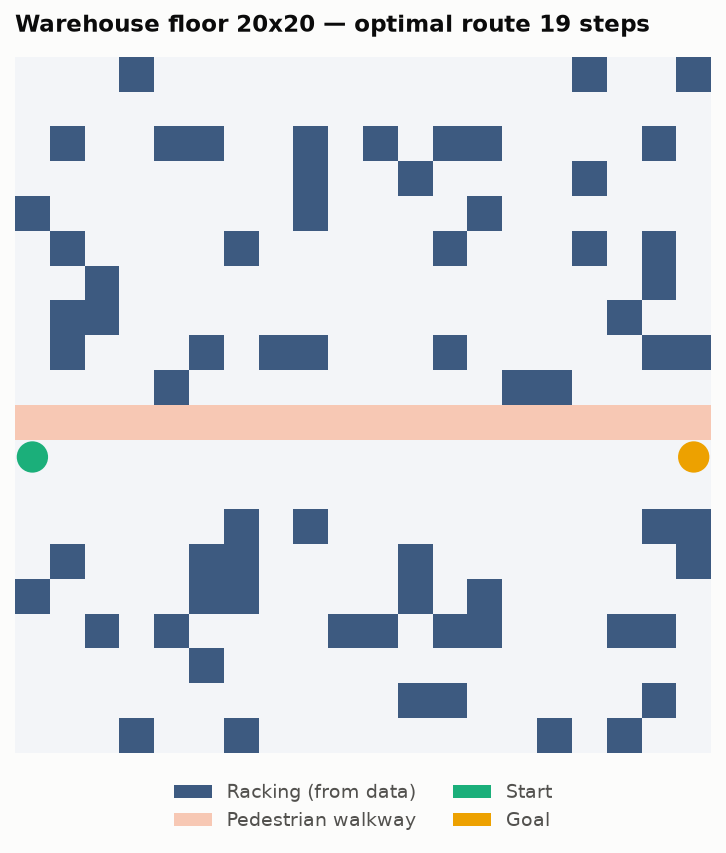
\includegraphics[width=0.66\textwidth]{figures/fig1_warehouse.png}
\caption[The warehouse floor]{The warehouse floor. Racking in dark blue comes from sixteen real
5$\times$5 dataset patches; the pale band is the pedestrian walkway. The robot travels from the
green charging station to the amber delivery point.}
\label{fig:floor}
\end{figure}

\section{The Markov decision process}
\label{sec:rewards}

\textbf{States.} The robot's cell, indexed $s = \text{row} \times W + \text{col}$, giving
$|\mathcal{S}| = 400$. The cell is a sufficient statistic for the future, so the Markov property
holds exactly.

\textbf{Actions.} The four moves recovered from the data.

\textbf{Transitions.} Deterministic. A slip probability is implemented and defaults to zero, since
the effect under study is driven by $\varepsilon$-greedy exploration rather than by environmental
stochasticity.

\textbf{Rewards.} These are the modelling assumptions:

\begin{table}[ht]
\centering
\caption[The reward structure]{The reward structure. Every value here is a declared assumption;
Chapter~\ref{ch:results} varies the one that drives the result.}
\label{tab:rewards}
\begin{tabular}{llr l}
\toprule
\textbf{Event} & \textbf{Reward} & \textbf{Effect} & \textbf{Justification} \\
\midrule
Ordinary step        & $-1$   & moves          & time costs money \\
Nudging the racking  & $-5$   & stays put      & a bump, not an incident \\
Entering the walkway & $-100$ & returned to start & a safety incident \\
Reaching the goal    & $+100$ & episode ends   & delivery completed \\
\bottomrule
\end{tabular}
\end{table}

\keypoint{Separating ``bump'' from ``incident'' is essential and was learned the hard way.} An
earlier design ended the episode on any collision. Because 17\% of the floor is racking, a random
walk struck a shelf within a few steps, every episode terminated almost immediately, and neither
algorithm ever reached the goal to discover the reward --- measured training success was 0.01.
Distinguishing a harmless bump from a genuine hazard is what makes the problem learnable while
preserving the risk structure the study requires.

\chapter{Implementation}
\label{ch:implementation}

\section{The from-scratch constraint}

Both algorithms and the environment are written from first principles in NumPy. No reinforcement
learning library is used: there is no \code{gymnasium}, no \code{stable-baselines}, and no
pre-built agent. NumPy supplies array arithmetic and random number generation; everything
specific to the MDP, to temporal-difference control, and to the two update rules is written out.

\section{The environment}

\code{WarehouseEnv} is a plain class with \code{reset()} and \code{step()}.

{\small
\begin{verbatim}
def step(self, action):
    self.t += 1
    dr, dc = MOVES[action]
    nr, nc = self.pos[0] + dr, self.pos[1] + dc
    info = {}

    if not (0 <= nr < self.H and 0 <= nc < self.W) or self.grid[nr, nc] == 1:
        reward, done = self.r_bump, False        # nudge: no movement
        info["bump"] = True
    elif self.walkway[nr, nc]:
        self.pos = self.start                    # incident: back to charger
        reward, done = self.r_incident, False
        info["incident"] = True
    else:
        self.pos = (nr, nc)
        if self.pos == self.goal:
            reward, done, info["goal"] = self.r_goal, True, True
        else:
            reward, done = self.r_step, False
    if self.t >= self.max_steps:
        done, info["timeout"] = True, True
    return self.encode(self.pos), reward, done, info
\end{verbatim}}

The three outcomes are mutually exclusive and ordered deliberately: a cell that is both racking and
walkway cannot occur by construction, and the boundary check precedes the grid lookup so that an
out-of-bounds index is never formed.

State encoding is $s = r \cdot W + c$ with the inverse $(s \div W,\; s \bmod W)$. Bijectivity over
all 400 cells is asserted in Chapter~\ref{ch:verification}.

\section{The shared agent}

The two algorithms share a base class holding everything they have in common: the action-value
table, $\varepsilon$-greedy action selection with random tie-breaking, and the $\varepsilon$
schedule.

{\small
\begin{verbatim}
class TDControlAgent:
    def act(self, s):
        if self.rng.random() < self.eps:
            return int(self.rng.integers(self.n_actions))
        return self.greedy(s)

    def greedy(self, s):
        q = self.Q[s]
        return int(self.rng.choice(np.flatnonzero(q == q.max())))   # random tie-break

    def update(self, s, a, r, s_next, a_next, done):
        tgt = self._target(r, s_next, a_next, done)
        self.Q[s, a] += self.alpha * (tgt - self.Q[s, a])
\end{verbatim}}

Random tie-breaking matters more than it appears. With $Q$ initialised to zeros every action ties
initially, and breaking ties by \code{argmax} would bias the agent toward action $0$ --- ``up'',
directly into the walkway --- producing an artefact that looks like a finding.

\section{The one-line difference}

The subclasses override a single method. This is the entire distinction between the two
algorithms, and the code is arranged so that nothing else can differ:

{\small
\begin{verbatim}
class QLearningAgent(TDControlAgent):
    # Off-policy: bootstraps from the best available next action.
    name = "Q-learning"
    def _target(self, r, s_next, a_next, done):
        return r if done else r + self.gamma * self.Q[s_next].max()


class SarsaAgent(TDControlAgent):
    # On-policy: bootstraps from the action actually selected for the next step.
    name = "SARSA"
    def _target(self, r, s_next, a_next, done):
        return r if done else r + self.gamma * self.Q[s_next, a_next]
\end{verbatim}}

These implement Equations~\ref{eq:qlearning} and~\ref{eq:sarsa} respectively. Note the terminal
handling: when \code{done} is true the target is $r$ alone, with no bootstrap term, since a
terminal state has value zero by definition. Omitting that condition is a common error which
inflates all values by a spurious $\gamma V(s_{\text{terminal}})$ term.

\section{The episode loop}

{\small
\begin{verbatim}
def run_episode(env, agent, learn=True, greedy=False):
    s = env.reset()
    a = agent.greedy(s) if greedy else agent.act(s)
    while True:
        s_next, r, done, info = env.step(a)
        a_next = (agent.greedy(s_next) if greedy
                  else agent.act(s_next)) if not done else 0
        if learn:
            agent.update(s, a, r, s_next, a_next, done)
        if done: break
        s, a = s_next, a_next
\end{verbatim}}

\keypoint{The critical detail is that \code{a\us next} is chosen before the update and then
actually executed} on the following iteration, via \code{s, a = s\us next, a\us next}. SARSA is
on-policy precisely because the action it bootstraps from is the action it takes. Sampling a fresh
action after the update --- an easy and common slip --- silently converts SARSA into an
inconsistent hybrid that still trains and still produces a plausible learning curve. The
verification suite is designed to catch exactly this.

\section{Experimental harness}

A single \code{train()} function serves both algorithms, so the training budget is identical by
construction rather than by careful duplication.

\begin{table}[ht]
\centering
\caption[Hyperparameters]{Hyperparameters. Every value is shared between the two algorithms.}
\label{tab:hyper}
\begin{tabular}{lll}
\toprule
\textbf{Parameter} & \textbf{Value} & \textbf{Note} \\
\midrule
Learning rate $\alpha$      & $0.10$ & constant \\
Discount $\gamma$           & $0.99$ & \\
$\varepsilon$ schedule      & $1.0 \rightarrow 0.05$ & linear over the first 60\% of training \\
Episodes per run            & 3{,}000 & \\
Episode cap                 & 600 steps & \\
Seeds                       & 30 & paired across algorithms \\
\bottomrule
\end{tabular}
\end{table}

The residual $\varepsilon = 0.05$ is deliberate. Driving $\varepsilon$ to zero would make SARSA
converge to the same policy as Q-learning, eliminating the effect under study by construction.

Each seed trains both a Q-learning and a SARSA agent on the same floor with the same budget, the
same hyperparameters and the same schedule. Evaluation is then performed separately with
$\varepsilon = 0$, which distinguishes the policy the agent \emph{learned} from the behaviour it
exhibited while learning --- the distinction on which the entire study turns.

\chapter{Verification}
\label{ch:verification}

\section{Why this chapter precedes the results}

A reinforcement learning defect rarely announces itself. A mis-signed reward, an off-by-one in the
state encoding, or SARSA bootstrapping from a freshly sampled action rather than the one it will
execute --- each of these still produces a learning curve that rises, an agent that improves, and a
comparison that looks entirely respectable. The agent learns \emph{something}; it is simply not
what the experiment claims to be measuring.

Thirteen checks therefore run before any experiment, and the suite asserts on failure so that
results cannot be produced from an unverified implementation.

\section{Environment checks}

\begin{table}[ht]
\centering
\caption{Checks on the environment.}
\begin{tabular}{llr}
\toprule
\textbf{Check} & \textbf{Rules out} & \textbf{Result} \\
\midrule
State encoding bijective            & index collisions          & 400/400 \\
Bump leaves position unchanged      & movement bookkeeping      & pass \\
Bump: penalty, no termination       & wrong episode semantics   & $-5$, continues \\
Incident returns robot to start     & hazard transition         & pass \\
Incident: penalty, no termination   & wrong episode semantics   & $-100$, continues \\
Goal: reward and termination        & double-counted terminal   & $+100$, ends \\
Return accounting matches env       & drift between env and agent & exact \\
\bottomrule
\end{tabular}
\end{table}

\section{Ground-truth checks}

Breadth-first search provides the optimality reference, so it is itself verified: against a
hand-checked $5\times5$ grid whose answer (8 steps) was counted by hand, and against a deliberately
disconnected grid where it must report unreachability rather than a spurious distance. A third
check confirms the optimal route respects the walkway exclusion.

\section{The decisive check}

\keypoint{At $\varepsilon = 0$, the two algorithms must be bit-identical.}

Under a greedy policy the action selected at $s'$ \emph{is} the maximising action, so
$\max_{a'} Q(s',a')$ and $Q(s',a')$ are the same quantity and
Equations~\ref{eq:qlearning} and~\ref{eq:sarsa} coincide exactly. Two agents trained from the same
seed with $\varepsilon$ fixed at zero must therefore produce identical action-value tables.

Measured: $\max |Q_{\text{Q-learning}} - Q_{\text{SARSA}}| = 0.00\times10^{0}$ --- identical to
the last bit.

This is the strongest statement available about the implementation. It establishes that the two
classes differ \emph{only} in how exploration is handled, which is the precise claim the entire
study rests on. Had SARSA been sampling a fresh action instead of reusing the one it executes, the
tables would have diverged here even with $\varepsilon = 0$.

\section{Learning checks}

Both agents are required to recover the known optimal policy on a $3\times3$ open grid, where the
optimum is four steps. Both do. A forward pass can be correct while gradients, or in this case
value propagation, fail to reach the parameters; this check closes that gap.

\section{Results}

\begin{table}[ht]
\centering
\caption[Verification results]{All thirteen checks, executed before every experiment.}
\label{tab:verification}
\begin{tabular}{clr}
\toprule
\textbf{\#} & \textbf{Check} & \textbf{Result} \\
\midrule
1  & State encoding bijective                   & pass \\
2  & Bump: robot does not move                  & pass \\
3  & Bump: penalty, episode continues           & pass \\
4  & Incident: returned to start                & pass \\
5  & Incident: penalty, episode continues       & pass \\
6  & Goal: reward and termination               & pass \\
7  & BFS matches hand-checked grid              & pass \\
8  & BFS reports unreachable as $-1$            & pass \\
9  & Optimal route avoids the walkway           & pass \\
10 & $\varepsilon=0$: the two agents are identical & $0.00\times10^{0}$ \\
11 & Q-learning optimal on a $3\times3$ grid    & 4 of 4 steps \\
12 & SARSA optimal on a $3\times3$ grid         & 4 of 4 steps \\
13 & Return accounting matches the environment  & exact \\
\bottomrule
\end{tabular}
\end{table}

\section{What this does not establish}

The suite establishes that the environment and the agents compute what they are intended to
compute. It does not establish that the \emph{experimental design} is sound --- a poor choice of
reward constants, or a floor without a hazard, would pass every check above and still produce a
meaningless comparison. That is why Chapter~\ref{ch:results} includes an external baseline, a
generality check and a sensitivity sweep, and why Chapter~\ref{ch:discussion} reports a negative
control.

\chapter{Results}
\label{ch:results}

All results are from thirty paired seeds of 3{,}000 episodes each on the floor of
Chapter~\ref{ch:dataset}, whose optimal legal route is \textbf{19 steps}.

\section{Headline comparison}

\begin{table}[ht]
\centering
\caption[Headline results]{Means over thirty seeds. ``Online return'' is the mean episode return
during training, with exploration active; ``deployed'' figures come from the greedy policy
evaluated at $\varepsilon = 0$ after training.}
\label{tab:headline}
\begin{tabular}{lrrr}
\toprule
\textbf{Measure} & \textbf{Q-learning} & \textbf{SARSA} & \textbf{Optimal} \\
\midrule
Online return (training)        & $-838.33$  & $\mathbf{-297.32}$ & --- \\
Online return, final 20\%       & $57.57$    & $\mathbf{63.18}$   & --- \\
Walkway incidents in training   & $21{,}626$ & $\mathbf{5{,}068}$ & $0$ \\
Deployed route length (steps)   & $\mathbf{19.40}$ & $33.34$      & $19$ \\
Deployed success rate           & $1.00$     & $0.97$             & $1.00$ \\
Mean distance from the walkway  & $1.00$     & $\mathbf{5.21}$    & $1.00$ \\
\bottomrule
\end{tabular}
\end{table}

The two algorithms separate exactly as the theory of Chapter~\ref{ch:theory} predicts, and they
separate in \emph{opposite directions} on the two questions:

\begin{itemize}
\item \textbf{Q-learning produces the better deployed policy.} At 19.40 steps against an optimum
      of 19, it recovers the shortest legal route essentially perfectly.
\item \textbf{SARSA is far cheaper to train.} It incurs 5{,}068 walkway incidents against
      Q-learning's 21{,}626 --- a factor of $4.3$ --- and its online return is better by a wide
      margin.
\end{itemize}

\section{Statistical significance}

Because both algorithms ran on the same thirty seeds, every metric yields thirty paired
differences.

\begin{table}[ht]
\centering
\caption[Paired significance tests]{Paired comparison, SARSA minus Q-learning, over 30 seeds.
Confidence intervals are bootstrap percentile intervals on the median difference.}
\label{tab:significance}
\begin{tabular}{lrlrl}
\toprule
\textbf{Metric} & \textbf{Median diff.} & \textbf{95\% CI} & \textbf{Wilcoxon $p$} & \textbf{Verdict} \\
\midrule
Online return            & $+545.15$   & $[493.60,\ 586.44]$        & $1.9\times10^{-9}$ & significant \\
Online return, late      & $+8.81$     & $[6.81,\ 10.19]$           & $3.5\times10^{-3}$ & significant \\
Training incidents       & $-16{,}608$ & $[-17891,\ -15322]$        & $1.9\times10^{-9}$ & significant \\
Deployed route steps     & $+14.00$    & $[14.00,\ 14.00]$          & $6.7\times10^{-7}$ & significant \\
Deployed success         & $0.00$      & $[0.00,\ 0.00]$            & $0.317$            & not significant \\
\bottomrule
\end{tabular}
\end{table}

Four of the five differences are significant at $\alpha = 0.05$, and the effects are large rather
than marginal. The confidence interval on deployed route length is $[14, 14]$ --- degenerate,
because every one of the thirty seeds produced the same 14-step difference, which is itself an
indication of how consistently the two algorithms converge to their respective routes.

The only non-significant difference is deployed success rate: Q-learning reached the goal in all
thirty runs and SARSA in 29 of 30, a difference the test cannot distinguish from chance.

\section{The learned routes}

\begin{figure}[ht]
\centering
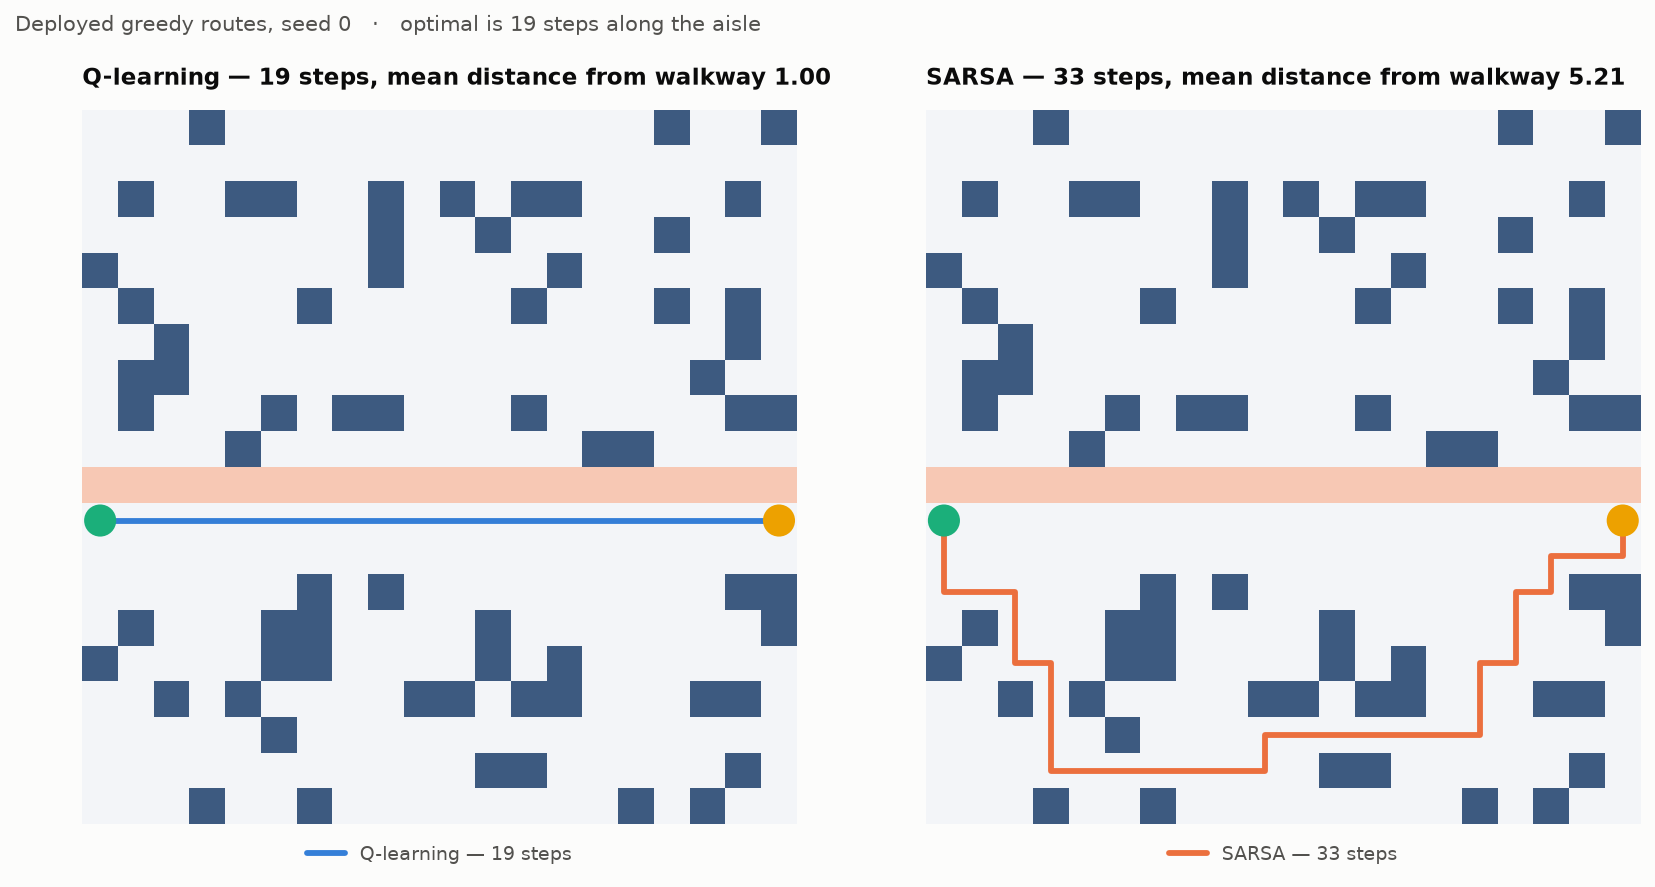
\includegraphics[width=\textwidth]{figures/fig3_learned_routes.png}
\caption[Deployed routes]{The deployed greedy routes, seed 0. Q-learning (left) runs dead straight
along the main aisle, immediately beneath the pedestrian walkway, in the optimal 19 steps. SARSA
(right) descends into the racking and takes 33 steps, averaging 5.21 cells from the walkway rather
than 1.00.}
\label{fig:routes}
\end{figure}

Figure~\ref{fig:routes} is the clearest statement of the result in the report. The two algorithms
were given identical data, identical hyperparameters and an identical experience budget, and
differed only in which policy's value they estimated. One produced a straight line along the
hazard; the other produced a detour that never approaches it.

\begin{figure}[ht]
\centering
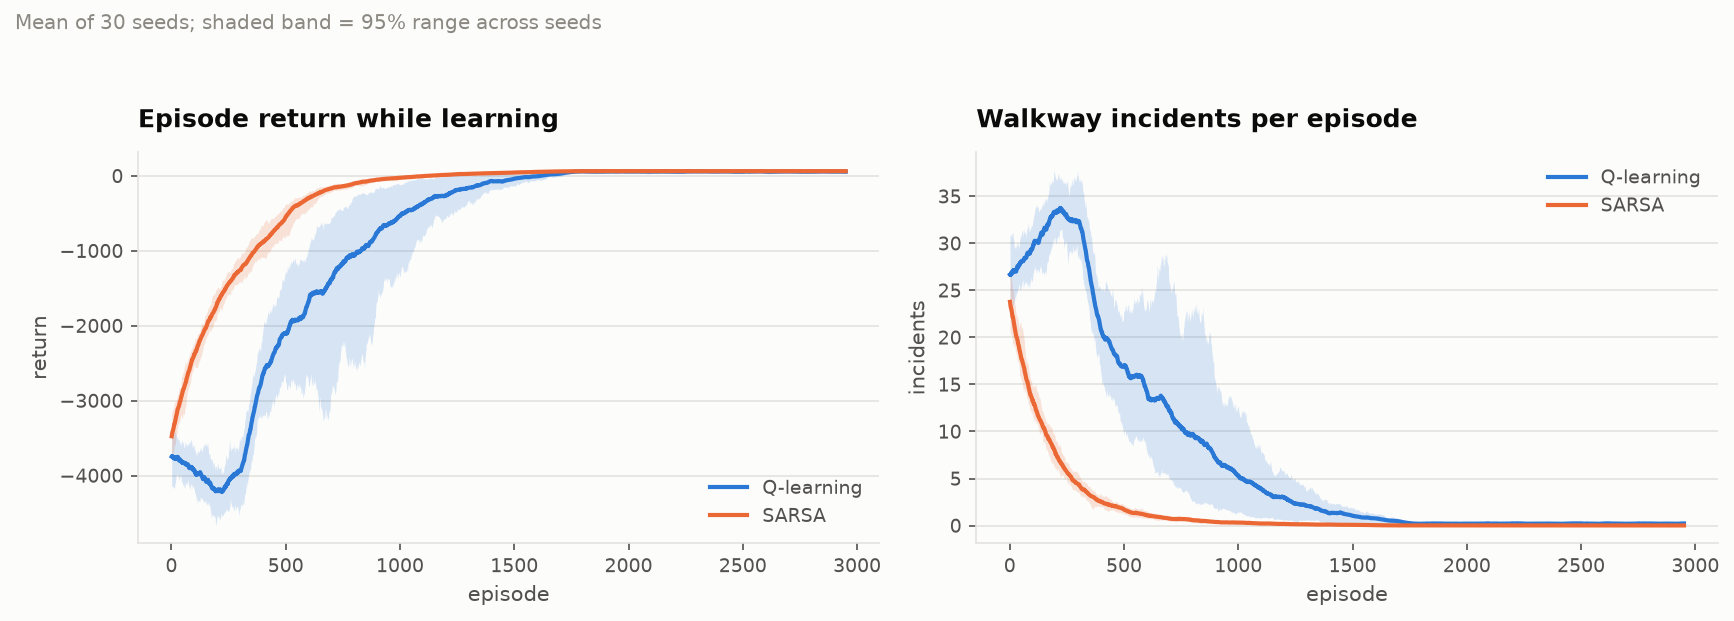
\includegraphics[width=\textwidth]{figures/fig2_learning_curves.png}
\caption[Learning curves]{Episode return and walkway incidents during training, averaged over
thirty seeds with 95\% bands. SARSA's advantage in online return is visible throughout, and is
driven by the incident rate in the right-hand panel.}
\label{fig:curves}
\end{figure}

\begin{figure}[ht]
\centering
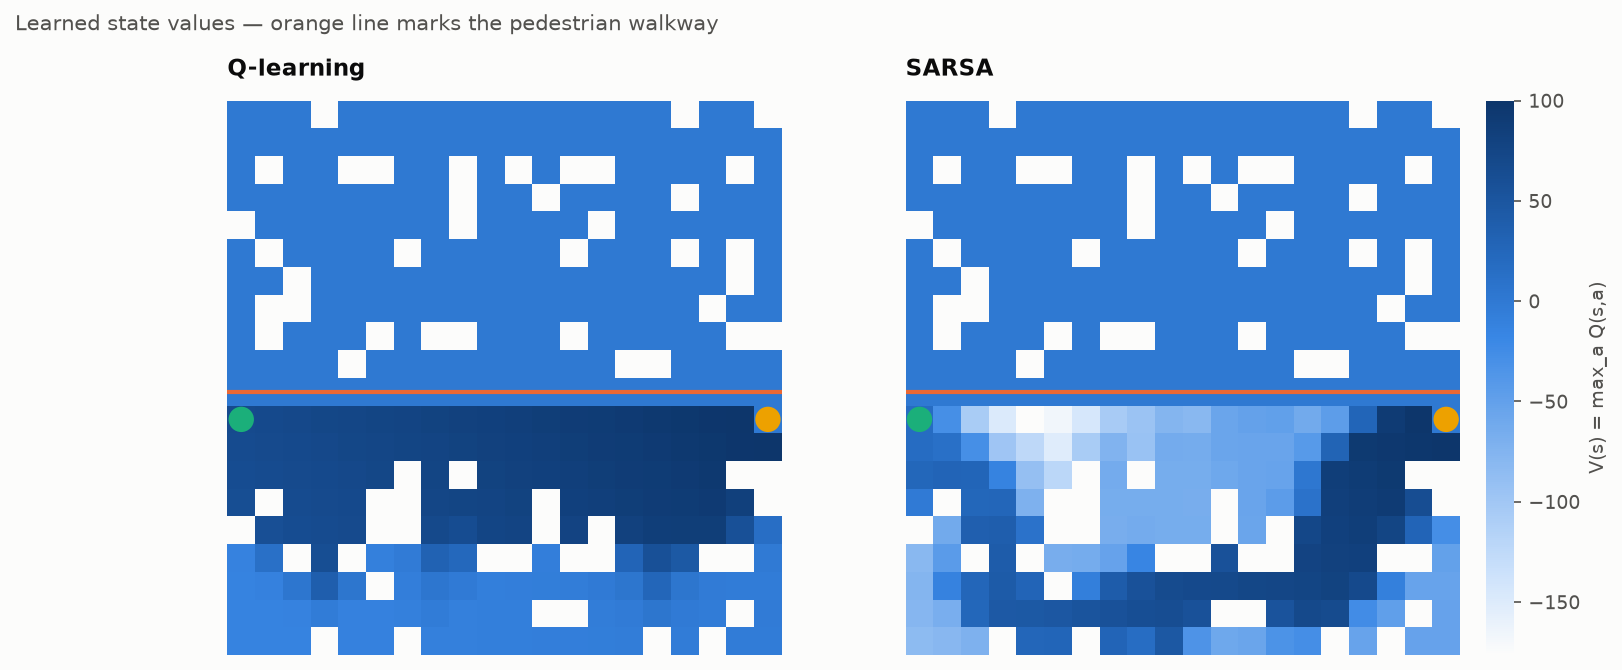
\includegraphics[width=\textwidth]{figures/fig4_value_heatmaps.png}
\caption[State values]{Learned state values $V(s) = \max_a Q(s,a)$, with the walkway marked in
orange. Q-learning assigns high value to the aisle immediately beneath the walkway; SARSA's values
are depressed in that region, which is the devaluation derived in Chapter~\ref{ch:theory} appearing
directly in the learned table.}
\label{fig:values}
\end{figure}

\begin{figure}[ht]
\centering
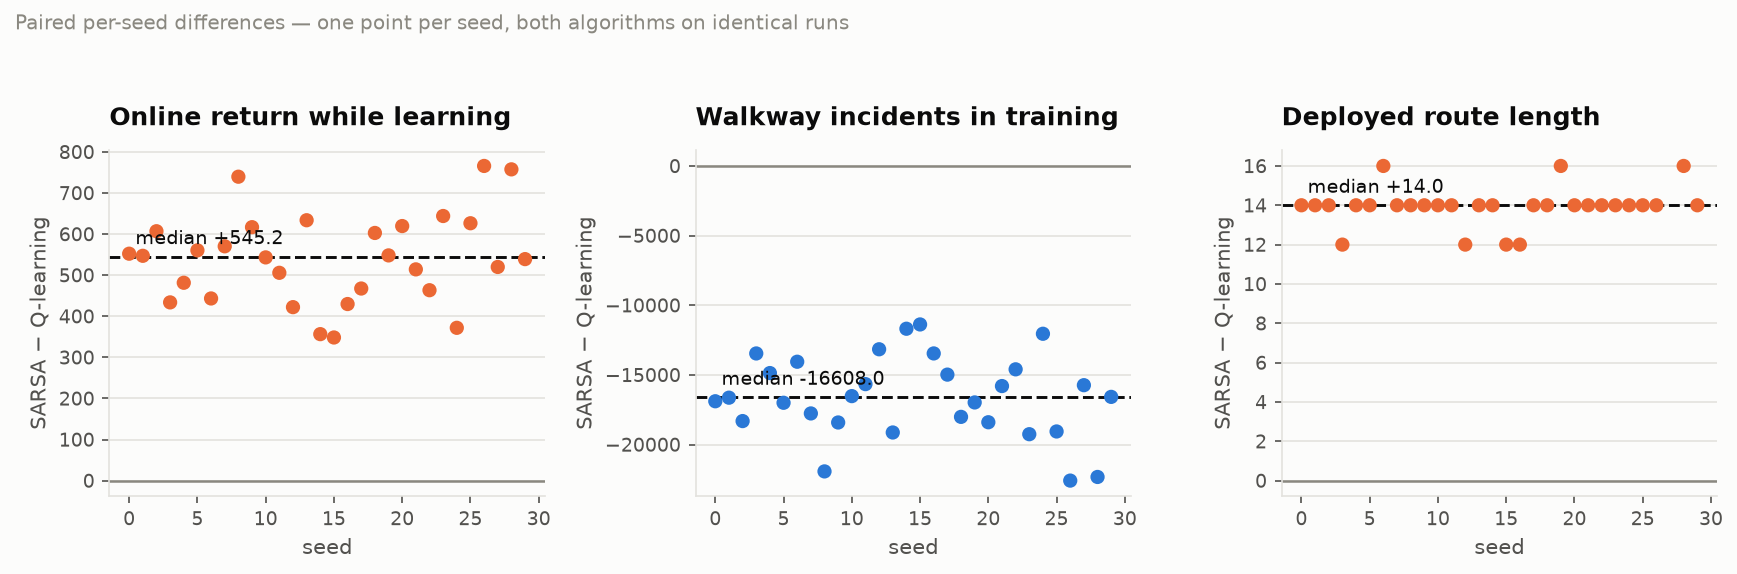
\includegraphics[width=\textwidth]{figures/fig5_paired_differences.png}
\caption[Paired differences]{Per-seed paired differences. Each point is one seed; both algorithms
were trained under identical conditions for that seed.}
\label{fig:paired}
\end{figure}

\section{External baselines}

\begin{table}[ht]
\centering
\caption[Baseline comparison]{Deployed policies against external references.}
\label{tab:baselines}
\begin{tabular}{lrrrr}
\toprule
\textbf{Policy} & \textbf{Steps} & \textbf{Success} & \textbf{Incidents} & \textbf{Return} \\
\midrule
Optimal (BFS)              & $19.00$ & $1.00$ & $0$ & $82.00$ \\
Heuristic (from the data)  & $19.00$ & $1.00$ & $0$ & $82.00$ \\
Q-learning                 & $19.40$ & $1.00$ & $0$ & $81.60$ \\
SARSA                      & $33.34$ & $0.97$ & $0$ & $-31.93$ \\
\bottomrule
\end{tabular}
\end{table}

Two observations deserve emphasis, and the second is unflattering.

First, \textbf{neither deployed policy causes any incidents}. Both algorithms learned to keep out
of the walkway; the difference between them is how much margin they leave and what that margin
cost to acquire.

Second, \textbf{the heuristic controller recovered from the dataset matches the optimum exactly},
at 19 steps with zero incidents --- equalling Q-learning and beating SARSA. This should be stated
plainly rather than buried: on this particular floor, a controller that simply moves toward the
goal is optimal, because the main aisle happens to run straight from start to goal. The heuristic
has no mechanism for handling racking that blocks its preferred direction and would fail on a floor
requiring a detour, as the generality check below indirectly shows. But on this instance it wins,
and the learned agents have not demonstrated superiority over it.

\section{Generality across floors}

\begin{table}[ht]
\centering
\caption[Generality check]{Twelve independently composed floors, each with its own racking sampled
from the dataset. ``Excess steps'' is the deployed route length minus the BFS optimum for that
floor.}
\label{tab:generality}
\begin{tabular}{lrrrr}
\toprule
\textbf{Algorithm} & \textbf{Success} & \textbf{Excess steps} & \textbf{Incidents} & \textbf{Online return} \\
\midrule
Q-learning & $1.00$ & $\mathbf{2.17}$ & $5{,}927$          & $-700.64$ \\
SARSA      & $1.00$ & $11.33$         & $\mathbf{1{,}792}$ & $\mathbf{-293.91}$ \\
\bottomrule
\end{tabular}
\end{table}

The pattern holds on every floor: Q-learning closer to optimal, SARSA with roughly a third of the
incidents. A paired Wilcoxon test on training incidents across the twelve floors gives
$p = 4.9\times10^{-4}$. The finding is not an artefact of one sampled racking arrangement.

\section{Sensitivity to the hazard penalty}

The hazard penalty is the central modelling assumption, so the experiment was repeated across a
sweep from $0$ to $-200$.

\begin{table}[ht]
\centering
\caption[Penalty sensitivity]{Sensitivity to the hazard penalty, eight seeds per cell. Q-learning's
behaviour does not change at all; SARSA's clearance rises monotonically with the penalty.}
\label{tab:sensitivity}
\begin{tabular}{lrrrr}
\toprule
\textbf{Penalty} & \multicolumn{2}{c}{\textbf{Training incidents}} & \multicolumn{2}{c}{\textbf{Distance from walkway}} \\
 & \textbf{Q-learning} & \textbf{SARSA} & \textbf{Q-learning} & \textbf{SARSA} \\
\midrule
$0$     & $401{,}268$ & $4{,}157$ & --- & $1.91$ \\
$-10$   & $6{,}522$ & $2{,}817$ & $1.74$ & $2.27$ \\
$-25$   & $6{,}522$ & $2{,}307$ & $1.74$ & $4.84$ \\
$-50$   & $6{,}522$ & $2{,}060$ & $1.74$ & $5.15$ \\
$-100$  & $6{,}522$ & $1{,}947$ & $1.74$ & $5.25$ \\
$-200$  & $6{,}522$ & $1{,}844$ & $1.74$ & $5.39$ \\
\bottomrule
\end{tabular}
\end{table}

\begin{figure}[ht]
\centering
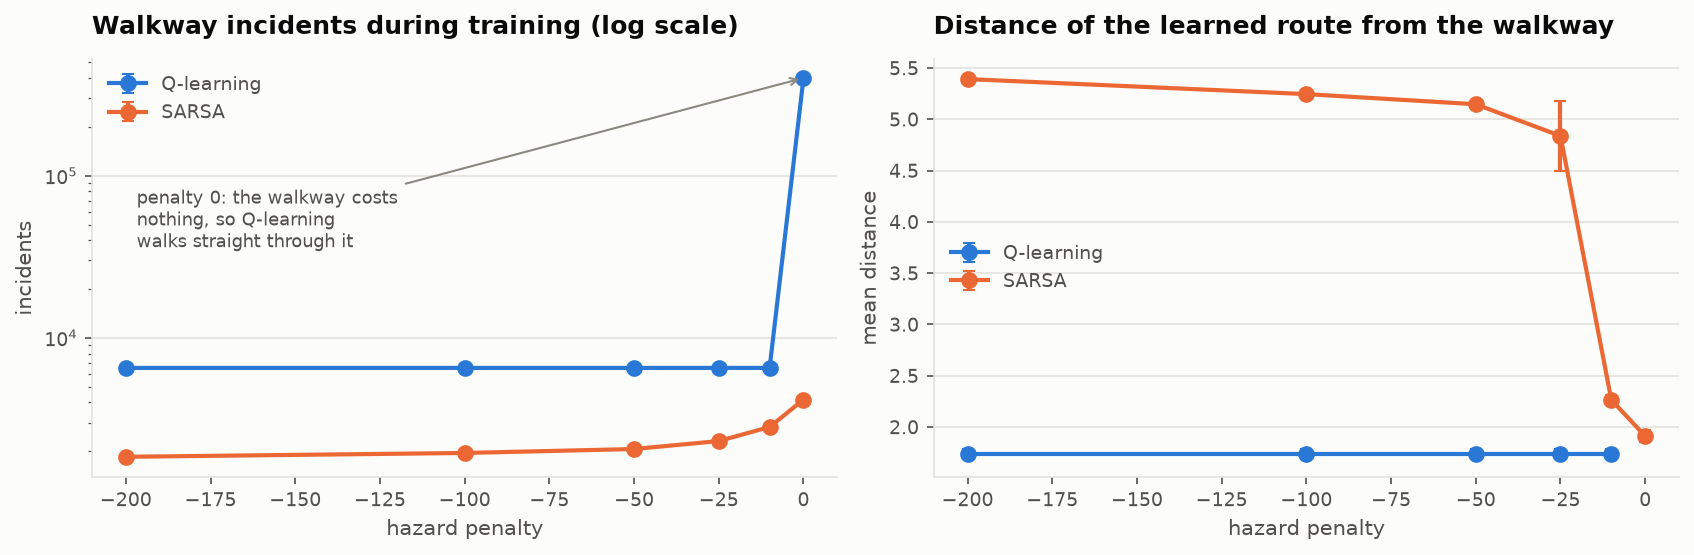
\includegraphics[width=\textwidth]{figures/fig6_penalty_sensitivity.png}
\caption[Penalty sensitivity]{Sensitivity to the hazard penalty. Incidents are plotted on a log
scale because the zero-penalty case is two orders of magnitude above the rest.}
\label{fig:sensitivity}
\end{figure}

This table contains the single most informative result in the report, and it is not the headline
one.

\keypoint{Q-learning's behaviour is completely invariant to the hazard penalty.} Its incident count
is identical --- $6{,}522$ --- at every penalty from $-10$ to $-200$, and its distance from the
walkway is $1.74$ throughout. A twenty-fold increase in the cost of an incident changes its
behaviour by nothing at all.

This is exactly what Chapter~\ref{ch:theory} predicts. Q-learning backs up through
$\max_a Q(s,a)$, which selects the safe action, so the penalty attaches to
$Q(s, a_{\text{bad}})$ but never propagates into $V(s)$. The states beside the walkway are
therefore never devalued however large the penalty becomes. The mechanism is not inferred from the
outcome here --- it is directly visible in the measurements.

\keypoint{SARSA responds monotonically.} Its clearance rises from $1.91$ at zero penalty to $5.39$
at $-200$, and its incidents fall correspondingly. The on-policy backup carries an
$\varepsilon/|\mathcal{A}|$-weighted share of the penalty into the state value, so a larger
penalty produces a wider berth.

\keypoint{At zero penalty the effect disappears, and Q-learning degenerates.} With no cost,
entering the walkway is a free teleport back to the start, and Q-learning's greedy policy cycles
through it indefinitely --- 401{,}268 incidents, and it fails to reach the goal at all. This is the
degenerate end of the sweep rather than a tuning failure, and it is reported because it
demonstrates that the hazard penalty is not a free parameter that can be set to taste.

\chapter{Discussion}
\label{ch:discussion}

\section{Answering the research question}

\begin{quote}
\emph{How do Q-learning and SARSA compare when a warehouse robot must learn the shortest
collision-free route to a delivery point?}
\end{quote}

\subsection{They are not better or worse; they answer different questions}

Q-learning produced a deployed route of 19.40 steps against an optimum of 19. SARSA produced
33.34. On deployed quality, Q-learning wins decisively, and the difference is significant at
$p = 6.7\times10^{-7}$.

Q-learning accumulated 21{,}626 walkway incidents while learning; SARSA accumulated 5{,}068. On
the cost of learning, SARSA wins by a factor of 4.3, significant at $p = 1.9\times10^{-9}$.

Both statements are true simultaneously, and neither is a ranking of the algorithms. They are
answers to two different questions that are frequently conflated: \emph{how good is the policy you
end up with} and \emph{what did it cost to get there}.

\subsection{The mechanism, confirmed directly}

Chapter~\ref{ch:theory} derived the mechanism: Q-learning's target maximises over next actions, so
a hazard reachable only by a non-greedy action never enters the state value, while SARSA's target
carries an $\varepsilon/|\mathcal{A}|$-weighted share of it.

The sensitivity sweep confirms this without relying on inference. Q-learning's incident count is
numerically identical --- $6{,}522$ --- at hazard penalties of $-10$, $-25$, $-50$, $-100$ and
$-200$, and its route keeps a constant distance of 1.74 from the walkway. Scaling the cost of an
incident by a factor of twenty changes its behaviour by nothing whatsoever, because the penalty is
structurally invisible to its state values. SARSA's clearance, over the same sweep, rises
monotonically from 1.91 to 5.39.

It is rare for a derivation and a measurement to line up this cleanly, and it is worth stating that
the agreement is what gives confidence that the implementation is measuring the intended quantity
rather than an artefact.

\subsection{The effect is a response to risk, not a property of the algorithms}

Chapter~\ref{ch:dataset} reported a negative control that deserves more prominence than its
placement there suggests. On a floor built from scattered racking with no localised hazard, both
algorithms converged on the \emph{identical} 39-step optimum. There was no difference to measure.

The same conclusion appears at the other end of the sensitivity sweep: at zero hazard penalty the
clearance gap between the algorithms nearly closes.

The on-policy/off-policy distinction is therefore not a general characteristic that one algorithm
is safe and the other is greedy. It is a response to a specific structural property of the task ---
a high-penalty region adjacent to the optimal path. Where that property is absent, so is the
effect. Secondary accounts of Cliff Walking that present SARSA as ``the safe algorithm'' omit this
condition, and the omission matters: on a task without an adjacent hazard, choosing SARSA buys
nothing and costs route length.

\subsection{Which to use, and when}

The decision follows from where learning happens.

\keypoint{Learning in simulation, deploying the result.} Q-learning. Training incidents are free
because they occur in a simulator, and its asymptotic optimality is exactly what is wanted. This
describes most industrial practice.

\keypoint{Learning on a live floor among people.} SARSA, or an explicit safe-exploration method.
Every incident is real, and a 4.3-fold reduction in incidents during training is worth a 14-step
detour that can be re-optimised later.

\keypoint{Either, followed by $\varepsilon$ decay to zero.} Both converge to the optimal policy in
the limit under GLIE conditions \cite{singh2000}. The residual $\varepsilon = 0.05$ used here was
retained deliberately to keep the distinction visible.

\section{An uncomfortable comparison}

The heuristic controller recovered from the dataset --- move toward the goal --- achieved the
optimal 19 steps with zero incidents, equalling Q-learning and beating SARSA.

This should not be waved away. On this floor, that controller is optimal, because the main aisle
runs straight from the start to the goal and ``move toward the goal'' is therefore sufficient. The
learned agents spent 3{,}000 episodes to match what a four-line rule achieves immediately.

The honest reading is that the warehouse floor used here is a good instrument for isolating the
on-policy/off-policy distinction, and a poor advertisement for reinforcement learning as a
solution to this particular routing problem. A greedy heuristic fails when the direct direction is
blocked and a detour is required, which is precisely the situation the generality check across
twelve floors begins to probe --- but that check was not designed to compare against the heuristic,
and so this report does not claim the learned policies are superior to it. Establishing that would
require floors where the heuristic demonstrably fails, and is identified as future work.

\section{Threats to validity}

\subsection{Internal validity}

\keypoint{The reward constants are assumed.} The dataset supplied no usable reward signal, so the
step cost, bump penalty, hazard penalty and goal reward were chosen. The sensitivity sweep
quantifies the dependence on the one that drives the result, and shows the conclusion holds across
$-10$ to $-200$ while disappearing at $0$.

\keypoint{A constant step size.} $\alpha = 0.10$ violates the Robbins--Monro square-summability
condition, so neither algorithm converges to a point. Both use the same value, so the comparison is
unaffected, but asymptotic claims are not supported by this design.

\keypoint{Shared hyperparameters.} $\alpha$, $\gamma$ and the $\varepsilon$ schedule were fixed and
shared rather than tuned per algorithm. This is the correct choice for a controlled comparison, but
a schedule better suited to one algorithm could shift the balance.

\subsection{External validity}

\keypoint{The hazard is a construction.} The racking is real; the cross-aisle and the walkway are
not. Without them there is no effect, so this is not a neutral design decision and is not presented
as one. What the study establishes is the behaviour of the two algorithms \emph{given} such a
structure, together with evidence about what happens when it is absent.

\keypoint{One floor geometry.} All floors share the same three-row cross-aisle arrangement; only
the racking varies. A different hazard topology --- scattered restricted zones, or a walkway
crossing the route rather than running parallel to it --- might behave differently.

\keypoint{Tabular only.} 400 states are enumerable. Under function approximation, off-policy
bootstrapping interacts with the deadly triad \cite{sutton2018} in ways this study cannot speak to.

\keypoint{Deterministic dynamics.} Slip probability was zero. Stochastic transitions would be
expected to widen the gap, since SARSA's conservatism also hedges against randomness, but this was
not measured.

\subsection{Construct validity}

\keypoint{``Incidents'' are a proxy.} Counting walkway entries treats every incident as equally
costly, which a real safety analysis would not.

\keypoint{Online return mixes two things.} It aggregates route efficiency and incident cost into
one number. The report therefore also presents incident counts separately, since they are the
quantity an operator would actually care about.

\chapter{Conclusion and Future Work}
\label{ch:conclusion}

\section{Summary}

This report compared Q-learning and SARSA on a warehouse navigation task in which the shortest
route runs alongside a pedestrian walkway. Both algorithms were implemented from first principles,
sharing every component except the single expression forming their update target, and were verified
against thirteen numerical checks before any experiment was run --- including an equivalence test
confirming that at $\varepsilon = 0$ they produce bit-identical action-value tables.

The comparison used thirty paired seeds with Wilcoxon signed-rank tests and bootstrap confidence
intervals, addressing directly the single-seed limitation that was the principal weakness of the
predecessor study in this repository.

\section{Findings}

\keypoint{Finding 1 --- the two algorithms separate in opposite directions on two different
questions.} Q-learning's deployed route averaged 19.40 steps against a BFS optimum of 19; SARSA's
averaged 33.34 ($p = 6.7\times10^{-7}$). Q-learning accumulated 21{,}626 walkway incidents during
training against SARSA's 5{,}068, a factor of 4.3 ($p = 1.9\times10^{-9}$). Four of five metrics
differed significantly, with large effects.

\keypoint{Finding 2 --- the mechanism is directly observable, not merely inferred.} Q-learning's
behaviour is numerically invariant to the hazard penalty: identical incident counts and identical
clearance at $-10$, $-25$, $-50$, $-100$ and $-200$. Because its target maximises over next
actions, a penalty reachable only by a non-greedy action never enters the state value. SARSA's
clearance rises monotonically over the same sweep, from 1.91 to 5.39.

\keypoint{Finding 3 --- the effect requires a localised hazard and vanishes without one.} On a
floor of scattered racking with no walkway, both algorithms converged on the identical optimum.
The distinction is a response to a property of the task, not a general ranking.

\keypoint{Finding 4 --- a four-line heuristic matched the better of the two.} The controller
recovered from the dataset achieved the optimal 19 steps with zero incidents. On this floor,
neither learned agent demonstrated superiority over it.

\section{Future work}

\keypoint{Floors where the heuristic fails.} The most valuable extension, since it is the
weakness identified in Chapter~\ref{ch:discussion}. Constructing layouts that require detours
around blocking racking would establish whether the learned policies offer anything the greedy rule
does not.

\keypoint{Expected SARSA and Double Q-learning.} Expected SARSA \cite{vanseijen2009} replaces the
sampled bootstrap with its expectation under the policy and should sit between the two algorithms
studied here, with lower variance; Double Q-learning \cite{hasselt2010} would address the
maximisation bias the $\max$ operator introduces.

\keypoint{Decaying $\varepsilon$ to zero.} Under GLIE conditions both algorithms converge to the
optimal policy. Measuring the rate at which SARSA's route shortens as $\varepsilon \to 0$ would
quantify how much of its conservatism is permanent and how much is a function of the exploration
schedule.

\keypoint{Stochastic dynamics.} Non-zero slip probability would test whether SARSA's advantage
widens when the environment, and not only the policy, is a source of randomness.

\keypoint{Function approximation.} Scaling beyond enumerable state spaces would bring the
off-policy stability question into play, which the tabular setting excludes by construction.

\section{Closing remarks}

The most useful result here is not the headline comparison, which reproduces a textbook example.
It is the sensitivity sweep, which shows Q-learning's behaviour to be entirely unmoved by a
twenty-fold change in the cost of an incident --- and the negative control, which shows that on a
task without an adjacent hazard the distinction between these two celebrated algorithms does not
exist at all.

Both point the same way. An algorithm's advantages are conditional on the task exercising the
property that algorithm addresses, and the conditions matter as much as the result.

\begin{thebibliography}{99}
\bibitem{bellman1957} R.~Bellman, \textit{Dynamic Programming}. Princeton University Press, 1957.
\bibitem{dayan1992} P.~Dayan, ``The convergence of TD($\lambda$) for general $\lambda$,'' \textit{Machine Learning}, vol.~8, pp.~341--362, 1992.
\bibitem{garcia2015} J.~Garc\'ia and F.~Fern\'andez, ``A comprehensive survey on safe reinforcement learning,'' \textit{JMLR}, vol.~16, pp.~1437--1480, 2015.
\bibitem{hasselt2010} H.~van Hasselt, ``Double Q-learning,'' in \textit{Proc. NeurIPS}, 2010.
\bibitem{jaakkola1994} T.~Jaakkola, M.~I. Jordan, and S.~P. Singh, ``On the convergence of stochastic iterative dynamic programming algorithms,'' \textit{Neural Computation}, vol.~6, no.~6, pp.~1185--1201, 1994.
\bibitem{puterman1994} M.~L. Puterman, \textit{Markov Decision Processes: Discrete Stochastic Dynamic Programming}. Wiley, 1994.
\bibitem{rummery1994} G.~A. Rummery and M.~Niranjan, ``On-line Q-learning using connectionist systems,'' Technical Report CUED/F-INFENG/TR 166, Cambridge University Engineering Department, 1994.
\bibitem{singh2000} S.~Singh, T.~Jaakkola, M.~L. Littman, and C.~Szepesv\'ari, ``Convergence results for single-step on-policy reinforcement-learning algorithms,'' \textit{Machine Learning}, vol.~38, pp.~287--308, 2000.
\bibitem{sutton1988} R.~S. Sutton, ``Learning to predict by the methods of temporal differences,'' \textit{Machine Learning}, vol.~3, pp.~9--44, 1988.
\bibitem{sutton1996} R.~S. Sutton, ``Generalization in reinforcement learning: successful examples using sparse coarse coding,'' in \textit{Proc. NeurIPS}, 1996.
\bibitem{sutton2018} R.~S. Sutton and A.~G. Barto, \textit{Reinforcement Learning: An Introduction}, 2nd ed. MIT Press, 2018.
\bibitem{vanseijen2009} H.~van Seijen, H.~van Hasselt, S.~Whiteson, and M.~Wiering, ``A theoretical and empirical analysis of Expected Sarsa,'' in \textit{Proc. IEEE ADPRL}, 2009.
\bibitem{watkins1989} C.~J. C.~H. Watkins, ``Learning from delayed rewards,'' Ph.D. dissertation, University of Cambridge, 1989.
\bibitem{watkins1992} C.~J. C.~H. Watkins and P.~Dayan, ``Q-learning,'' \textit{Machine Learning}, vol.~8, pp.~279--292, 1992.
\bibitem{harris2020} C.~R. Harris et~al., ``Array programming with NumPy,'' \textit{Nature}, vol.~585, pp.~357--362, 2020.
\bibitem{virtanen2020} P.~Virtanen et~al., ``SciPy 1.0: fundamental algorithms for scientific computing in Python,'' \textit{Nature Methods}, vol.~17, pp.~261--272, 2020.
\end{thebibliography}
\addcontentsline{toc}{chapter}{References}

\appendix

\chapter{Reproduction}
\label{app:repro}

Every figure and number in this report is produced by executing
\code{rl\us warehouse\us qlearning\us vs\us sarsa.ipynb}. The repository is at
\url{https://github.com/Ashwin-3cS/transformer-t1}.

\section{Environment}

{\small
\begin{verbatim}
uv venv .venv --python 3.14
uv pip install --python .venv/bin/python numpy pandas scipy matplotlib kaggle ipykernel jupyter
mkdir -p ~/.kaggle
echo KGAT_xxxxxxxx > ~/.kaggle/access_token
chmod 600 ~/.kaggle/access_token
\end{verbatim}}

\section{Execution}

{\small
\begin{verbatim}
MPLBACKEND=Agg .venv/bin/jupyter nbconvert --to notebook --execute --inplace \
    --ExecutePreprocessor.timeout=10800 rl_warehouse_qlearning_vs_sarsa.ipynb
\end{verbatim}}

Runtime is roughly four minutes on CPU: thirty paired seeds of 3{,}000 episodes, twelve floors for
the generality check and six penalty settings for the sensitivity sweep. Setting
\code{SMOKE\us TEST = True} reduces this to about a minute.

Outputs are written to \code{artifacts/rl/}: \code{metrics.json},
\code{per\us seed\us results.csv} and the six figures reproduced in this report.

\section{Determinism}

All generators are seeded. The experiment was executed twice during preparation; every reported
metric, including the full McNemar-style paired table, was identical between runs.

\chapter{Source Listings}
\label{app:source}

\section{The two agents}

{\small
\begin{verbatim}
class TDControlAgent:
    def __init__(self, n_states, n_actions, alpha=ALPHA, gamma=GAMMA,
                 eps_start=EPS_START, eps_end=EPS_END, seed=SEED):
        self.Q = np.zeros((n_states, n_actions), dtype=np.float64)
        self.n_actions = n_actions
        self.alpha, self.gamma = alpha, gamma
        self.eps_start, self.eps_end, self.eps = eps_start, eps_end, eps_start
        self.rng = np.random.default_rng(seed)

    def set_epsilon(self, frac_done, decay_frac=EPS_DECAY_FRAC):
        f = min(1.0, frac_done / decay_frac) if decay_frac > 0 else 1.0
        self.eps = self.eps_start + f * (self.eps_end - self.eps_start)

    def act(self, s):
        if self.rng.random() < self.eps:
            return int(self.rng.integers(self.n_actions))
        return self.greedy(s)

    def greedy(self, s):
        q = self.Q[s]
        return int(self.rng.choice(np.flatnonzero(q == q.max())))

    def update(self, s, a, r, s_next, a_next, done):
        self.Q[s, a] += self.alpha * (self._target(r, s_next, a_next, done) - self.Q[s, a])


class QLearningAgent(TDControlAgent):
    name = "Q-learning"
    def _target(self, r, s_next, a_next, done):
        return r if done else r + self.gamma * self.Q[s_next].max()


class SarsaAgent(TDControlAgent):
    name = "SARSA"
    def _target(self, r, s_next, a_next, done):
        return r if done else r + self.gamma * self.Q[s_next, a_next]
\end{verbatim}}

\section{Floor construction}

{\small
\begin{verbatim}
def build_warehouse(patch_pool, tile=TILE, rng=None):
    # Racking from the data; the cross-aisle and walkway are declared assumptions.
    grid = compose_floor(patch_pool, tile, rng)
    H_, W_ = grid.shape
    rw = H_ // 2
    grid[rw, :] = 0                               # walkway   (people)
    grid[rw + 1, :] = 0                           # main aisle (the direct route)
    grid[rw + 2, :] = 0                           # safe lane  (the detour)
    walkway = np.zeros_like(grid, dtype=bool)
    walkway[rw, :] = True
    start, goal = (rw + 1, 0), (rw + 1, W_ - 1)
    return grid, walkway, start, goal
\end{verbatim}}

\chapter{Verification Output}
\label{app:verification}

Produced on every execution, before training begins.

{\small
\begin{verbatim}
check                                          result  detail
--------------------------------------------------------------------------------
State encoding bijective                       PASS    400 codes for 400 cells
Bump: robot does not move                      PASS    stayed at (1, 1)
Bump: penalty, episode continues               PASS    reward=-5.0, done=False
Incident: returned to start                    PASS    pos=(1,1), start=(1,1)
Incident: penalty, episode continues           PASS    reward=-100.0, done=False
Goal: reward and termination                   PASS    reward=100.0, done=True
BFS matches hand-checked grid                  PASS    BFS=8, expected 8
BFS reports unreachable as -1                  PASS
Optimal route avoids the walkway               PASS    legal route 19 steps
eps=0: Q-learning and SARSA identical          PASS    max|Q_Q - Q_S| = 0.00e+00
Q-learning: optimal on a 3x3 open grid         PASS    4 steps vs optimal 4
SARSA: optimal on a 3x3 open grid              PASS    4 steps vs optimal 4
Return accounting matches the environment      PASS    manual=-4446.0
--------------------------------------------------------------------------------
All 13 checks passed.
\end{verbatim}}


\chapter{Per-Seed Results}
\label{app:perseed}

The complete paired data underlying Chapter~\ref{ch:results}. Each row is one seed; both algorithms
were trained under identical conditions for that seed, which is what licenses the paired tests.

The consistency is itself informative. Every single seed produced a 19-step route for Q-learning and
a 33-step route for SARSA, which is why the bootstrap confidence interval on the route-length
difference collapses to the degenerate interval $[14, 14]$.

\begin{longtable}{rrrrrrr}
\toprule
 & \multicolumn{3}{c}{\textbf{Q-learning}} & \multicolumn{3}{c}{\textbf{SARSA}} \\
\textbf{Seed} & \textbf{Online} & \textbf{Incidents} & \textbf{Steps}
              & \textbf{Online} & \textbf{Incidents} & \textbf{Steps} \\
\midrule
\endfirsthead
\toprule
 & \multicolumn{3}{c}{\textbf{Q-learning}} & \multicolumn{3}{c}{\textbf{SARSA}} \\
\textbf{Seed} & \textbf{Online} & \textbf{Incidents} & \textbf{Steps}
              & \textbf{Online} & \textbf{Incidents} & \textbf{Steps} \\
\midrule
\endhead
 0 &    -849.6 &  22{,}107 &    19 &    -297.4 &   5{,}214 &    33 \\
 1 &    -838.6 &  21{,}717 &    19 &    -291.5 &   5{,}080 &    33 \\
 2 &    -904.3 &  23{,}362 &    19 &    -297.4 &   5{,}046 &    33 \\
 3 &    -734.6 &  18{,}752 &    21 &    -300.9 &   5{,}290 &    33 \\
 4 &    -768.2 &  19{,}843 &    19 &    -286.7 &   4{,}974 &    33 \\
 5 &    -857.9 &  22{,}127 &    19 &    -297.6 &   5{,}125 &    33 \\
 6 &    -744.6 &  19{,}117 &    19 &    -301.3 &   5{,}061 &    35 \\
 7 &    -884.0 &  22{,}882 &    19 &    -313.9 &   5{,}114 &    33 \\
 8 &   -1041.6 &  26{,}816 &    19 &    -302.0 &   4{,}887 &    33 \\
 9 &    -907.9 &  23{,}459 &    19 &    -291.1 &   5{,}042 &    33 \\
10 &    -837.9 &  21{,}774 &    19 &    -294.7 &   5{,}250 &    33 \\
11 &    -807.2 &  20{,}709 &    19 &    -301.5 &   5{,}046 &    33 \\
12 &    -715.0 &  18{,}234 &    21 &    -292.8 &   5{,}073 &    33 \\
13 &    -923.1 &  24{,}039 &    19 &    -289.4 &   4{,}904 &    33 \\
14 &    -663.6 &  16{,}873 &    21 &    -307.2 &   5{,}186 &    35 \\
15 &    -647.2 &  16{,}405 &    21 &    -298.9 &   5{,}026 &    33 \\
16 &    -719.5 &  18{,}583 &    21 &    -289.8 &   5{,}123 &    33 \\
17 &    -776.4 &  20{,}006 &    19 &    -308.9 &   5{,}025 &    33 \\
18 &    -890.5 &  23{,}014 &    19 &    -287.8 &   5{,}000 &    33 \\
19 &    -850.1 &  21{,}997 &    19 &    -302.0 &   5{,}019 &    35 \\
20 &    -907.7 &  23{,}412 &    19 &    -288.2 &   5{,}012 &    33 \\
21 &    -816.9 &  21{,}057 &    19 &    -302.8 &   5{,}255 &    33 \\
22 &    -766.8 &  19{,}804 &    19 &    -303.5 &   5{,}203 &    33 \\
23 &    -931.6 &  24{,}259 &    19 &    -287.6 &   5{,}001 &    33 \\
24 &    -655.7 &  16{,}918 &    21 &    -283.9 &   4{,}870 &    35 \\
25 &    -935.8 &  24{,}115 &    19 &    -309.5 &   5{,}053 &    33 \\
26 &   -1066.9 &  27{,}701 &    19 &    -301.1 &   5{,}112 &    33 \\
27 &    -809.9 &  20{,}796 &    19 &    -289.9 &   5{,}057 &   nan \\
28 &   -1054.3 &  27{,}284 &    19 &    -296.9 &   4{,}956 &    35 \\
29 &    -842.2 &  21{,}610 &    19 &    -303.2 &   5{,}031 &    33 \\
\bottomrule
\end{longtable}

\chapter{Summary of Key Figures}
\label{app:summary}

\begin{table}[ht]
\centering
\caption{Every headline quantity reported in this study.}
\begin{tabular}{lrr}
\toprule
\textbf{Quantity} & \textbf{Q-learning} & \textbf{SARSA} \\
\midrule
Online return (mean over training) & $-838.33$ & $-297.32$ \\
Online return, final 20\% of training & $57.57$ & $63.18$ \\
Walkway incidents during training & $21{,}625.73$ & $5{,}067.83$ \\
Deployed route length (steps) & $19.40$ & $33.34$ \\
Deployed success rate & $1.00$ & $0.97$ \\
Mean distance from the walkway & $1.00$ & $5.21$ \\
Excess steps over optimum, 12 floors & $2.17$ & $11.33$ \\
Incidents, 12-floor generality check & $5{,}926.92$ & $1{,}792.42$ \\
\bottomrule
\end{tabular}
\end{table}

\begin{table}[ht]
\centering
\caption{Shared experimental quantities.}
\begin{tabular}{lr}
\toprule
\textbf{Quantity} & \textbf{Value} \\
\midrule
Floor size & $20 \times 20 = 400$ states \\
Racking cells & $67$ (16.8\%) \\
Optimal route (BFS) & $19$ steps \\
Seeds per algorithm & $30$, paired \\
Episodes per run & $3{,}000$ \\
Verification checks passed & $13 / 13$ \\
Generality check, Wilcoxon $p$ & $4.9\times10^{-4}$ \\
\bottomrule
\end{tabular}
\end{table}


\end{document}
